\documentclass[nynorsk,12pt,a4paper]{article}
\usepackage[utf8]{inputenc}
\usepackage[T1]{fontenc}
\usepackage{graphicx}
\usepackage{babel}
\renewcommand*{\familydefault}{\rmdefault}
\title{Kravdokument\\
Dynamisk Nettverksbrannmur
}
\author{Espen Gjærde \and Svein Ove Undal}
\date{09.04.2013}

\pagenumbering{arabic}
\begin{document}
\maketitle

\newpage
\section*{Revisjonshistorie}
\begin{table}[h!]
	\begin{tabular}{ l l l l }

		\textsc{Dato} & \textsc{Versjon} & \textsc{Forklaring} & \textsc{Forfattar} \\
		\hline 
		18.02.2013 & 1.0 & Dokumentet opprettet & Espen \\ 
		04.04.2013 & 1.1 & Kapittel 1 og 3 på plass & Espen \\ 
		08.04.2013 & 1.2 & Tabellar UC og SSD & Espen \\ 
		\hline
	\end{tabular}
\end{table}

\newpage
\tableofcontents

\newpage
\section{Innleiing}
\subsection{Hensikta med dokumentet}
\paragraph{}
Hensikta med dette dokumentet er å gi ei oversikt over krava som vert stilt til bruk systemet, og eventuelle tilleggsfunksjonar som er ønska. Dokumentet sin viktigaste funksjon er å skildre systemet og systemet sitt grensesnitt. Dette blir gjort ved bruk av standardiserte logiske modellar. 

\subsection{Avgrensingar}
\paragraph{}
Innhaldet i dette dokumentet skildrar den funksjonaliteten som produktet gir, samt det som vi har programmert,  men ikkje funksjonaliteten til dei linux-modulane som produktet nyttar seg av. 

\subsection{Definisjonar og forkortingar}
\paragraph{}
Som definert i kapittel 8.3.4 i Visjonsdokumentet nyttar vi nynorsk i skriftleg dokumentasjon, men engelsk i all kode og alle kodekommentarar. Det kan derfor skje at vi refererer til det engelske navnet <<Dynamic Network Firewall>> eller <<DNF>> også i den norske dokumentasjonen.

\subsection{Referansar}
\paragraph{}
Visjonsdokument versjon 1.2, side 15

\subsection{Oversikt over innhald}
\paragraph{}
Dette dokumentet har i alt fem kapittel. I første kapittel vert bakgrunn og grunnlag for sjølve dokumentet forklart. Vidare vil kapittel to og tre ta for seg use caser der dei først blir skildra med logiske modellar, og deretter skriftlig forklart. I kapittel fem går vi gjennom dei same usecasane frå systemet sin ståstad og fokuserer meir på det tekniske. 

\newpage
\section{Bakgrunn og oversikt}
\subsection{Use Case -- UML-diagram}
\includegraphics[scale=0.5]{gfx/UC.eps} 
\newpage
\section{Detaljerte krav}
\subsection{Use Case: Logg inn} 
\begin{table}[h!]
	\begin{tabular}{l p{10cm}}
		\textsc{Namn} & Logg inn \\
		\textsc{Mål} & Authentisere brukarar og gi tilgang gjennom brannmuren \\
		\textsc{Aktør} & Brukar, administrator \\
		\textsc{Utløysar} & Brukar koplar seg til internett før pålogging \\
		\textsc{Føresetnad} & Brukaren er ikkje pålogga \\
		\textsc{Effekt} & Brukaren får tilgang til ressursar bak brannmuren, vert innlogga. \\
		\textsc{Hovudløp} & 
			\begin{enumerate} \itemsep1pt \parskip0pt \parsep0pt
				\item \uppercase{logg inn}
			\end{enumerate}				
		 \\
		\textsc{Relaterte løp} & Ingen \\
		\textsc{Unntak} & Ingen \\
		\textsc{Tilleggsinformasjon} & Ingen \\	
	\end{tabular}
\end{table}

\subsection{Use Case: Vis statistikk} 
\begin{table}[h!]
	\begin{tabular}{l p{10cm}}
		\textsc{Namn} & Vis statistikk \\
		\textsc{Mål} & Vise brukaren statistikk over sin nettbruk, informere om eventuelle avgrensingar sett for brukaren. \\
		\textsc{Aktør} & Brukar, administrator \\
		\textsc{Utløysar} & Ingen \\
		\textsc{Føresetnad} & Brukaren er logga inn \\
		\textsc{Effekt} & Ingen \\
		\textsc{Hovudløp} & 
			\begin{enumerate} \itemsep1pt \parskip0pt \parsep0pt
				\item \uppercase{vis statistikk}
			\end{enumerate}				
		 \\
		\textsc{Relaterte løp} & Ingen \\
		\textsc{Unntak} & Ingen \\
		\textsc{Tilleggsinformasjon} & Ingen \\	
	\end{tabular}
\end{table}

\newpage
\subsection{Use Case: Administrer brannmur}  
\begin{table}[h!]
	\begin{tabular}{l p{10cm}}
		\textsc{Namn} & Administrere brannmur \\
		\textsc{Mål} & Manuelt sette eller oppdatere avgrensing og reglar i brannmuren \\
		\textsc{Aktør} & Administrator \\
		\textsc{Utløysar} & Ingen \\
		\textsc{Føresetnad} & Pålogga som administrator \\
		\textsc{Effekt} & Brannmuren vert oppdatert \\
		\textsc{Hovudløp} & 
			\begin{enumerate} \itemsep1pt \parskip0pt \parsep0pt
				\item \uppercase{hent reglar}
				\item \uppercase{gjenta 3-5 så lenge brukaren ønsker}
				\item \uppercase{eller: endre regel}
				\item \uppercase{eller: lag regel}
				\item \uppercase{eller: slett regel}
				\item \uppercase{oppdater brannmur}
			\end{enumerate}				
		 \\
		\textsc{Relaterte løp} & Ingen \\
		\textsc{Unntak} & Ingen \\
		\textsc{Tilleggsinformasjon} & Ingen \\	
	\end{tabular}
\end{table}

\newpage
\section{Systemsekvensdiagram}
\subsection{Use Case: Logg inn}
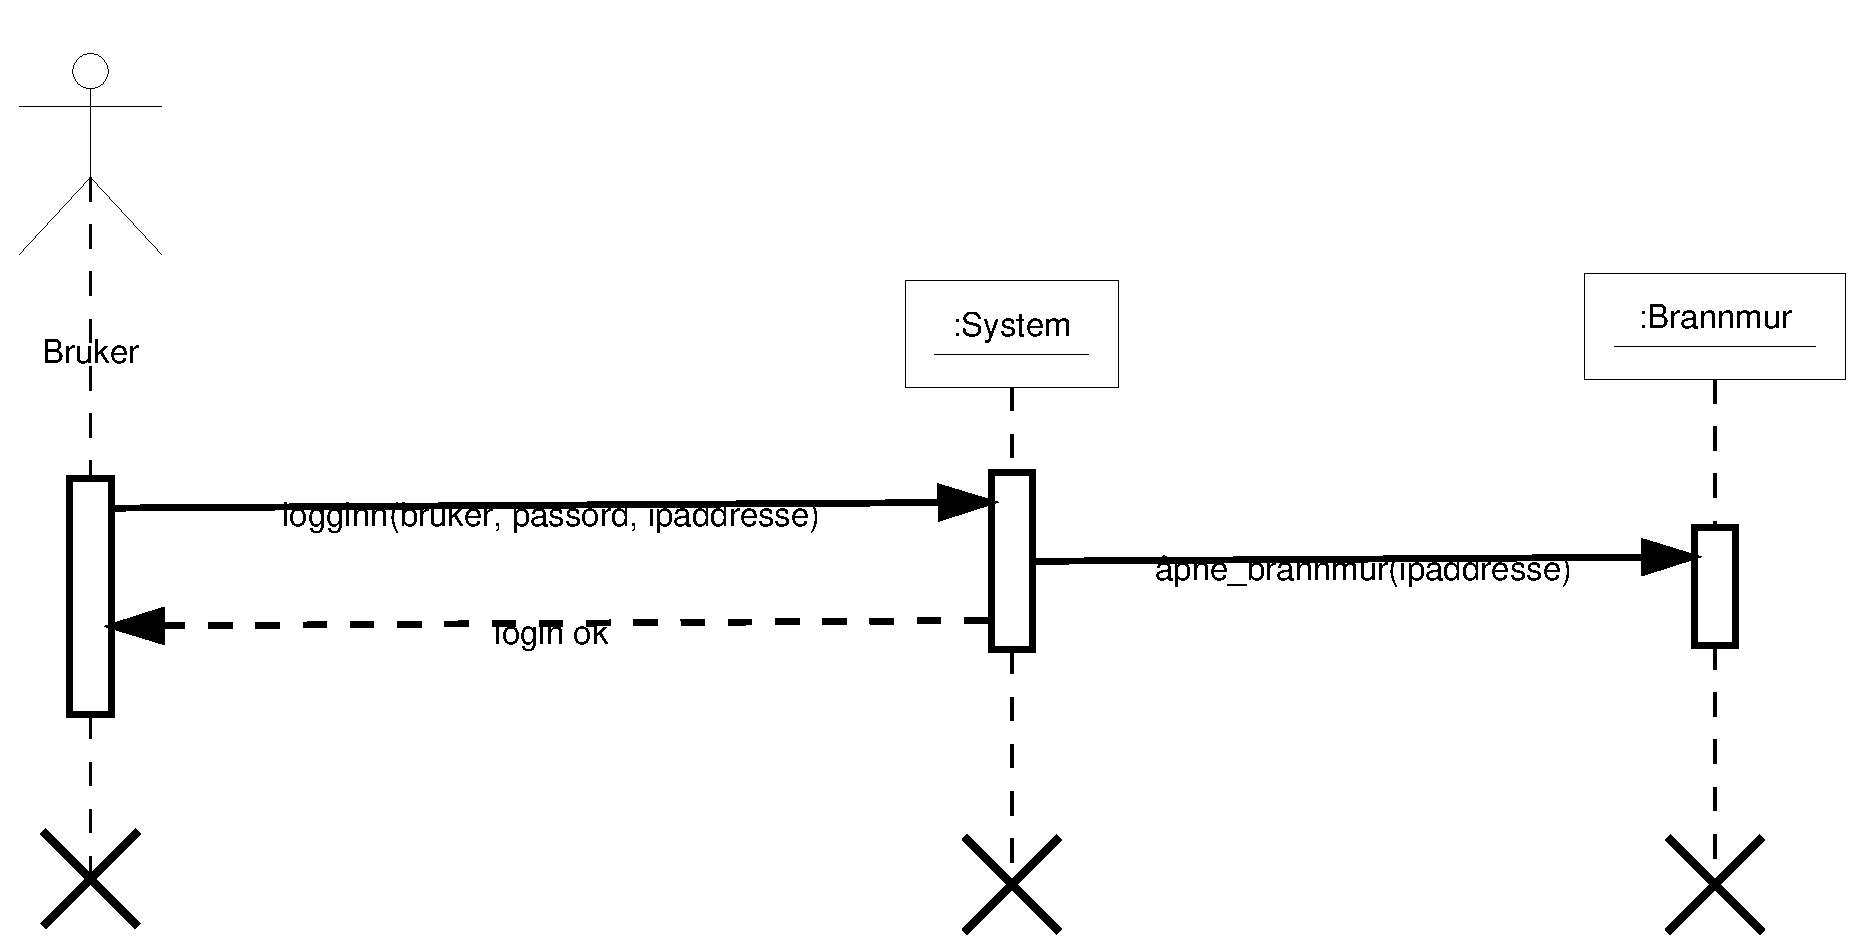
\includegraphics[scale=0.5]{gfx/SSD_UC1_login.eps}
\subsection{Use Case: Vis statistikk}
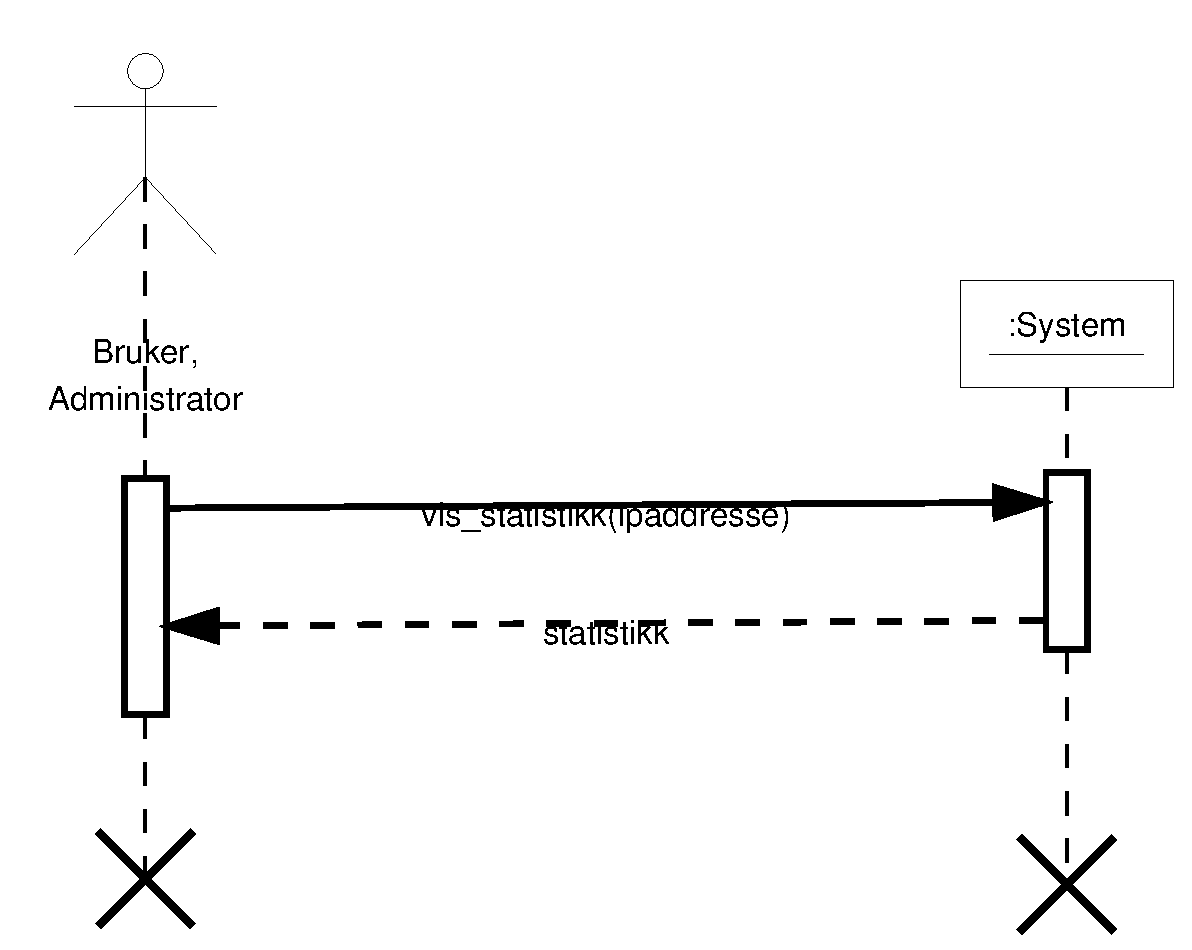
\includegraphics[scale=0.5]{gfx/SSD_UC2_vis_statistikk.eps}
\subsection{Use Case: Administrere brannmur}
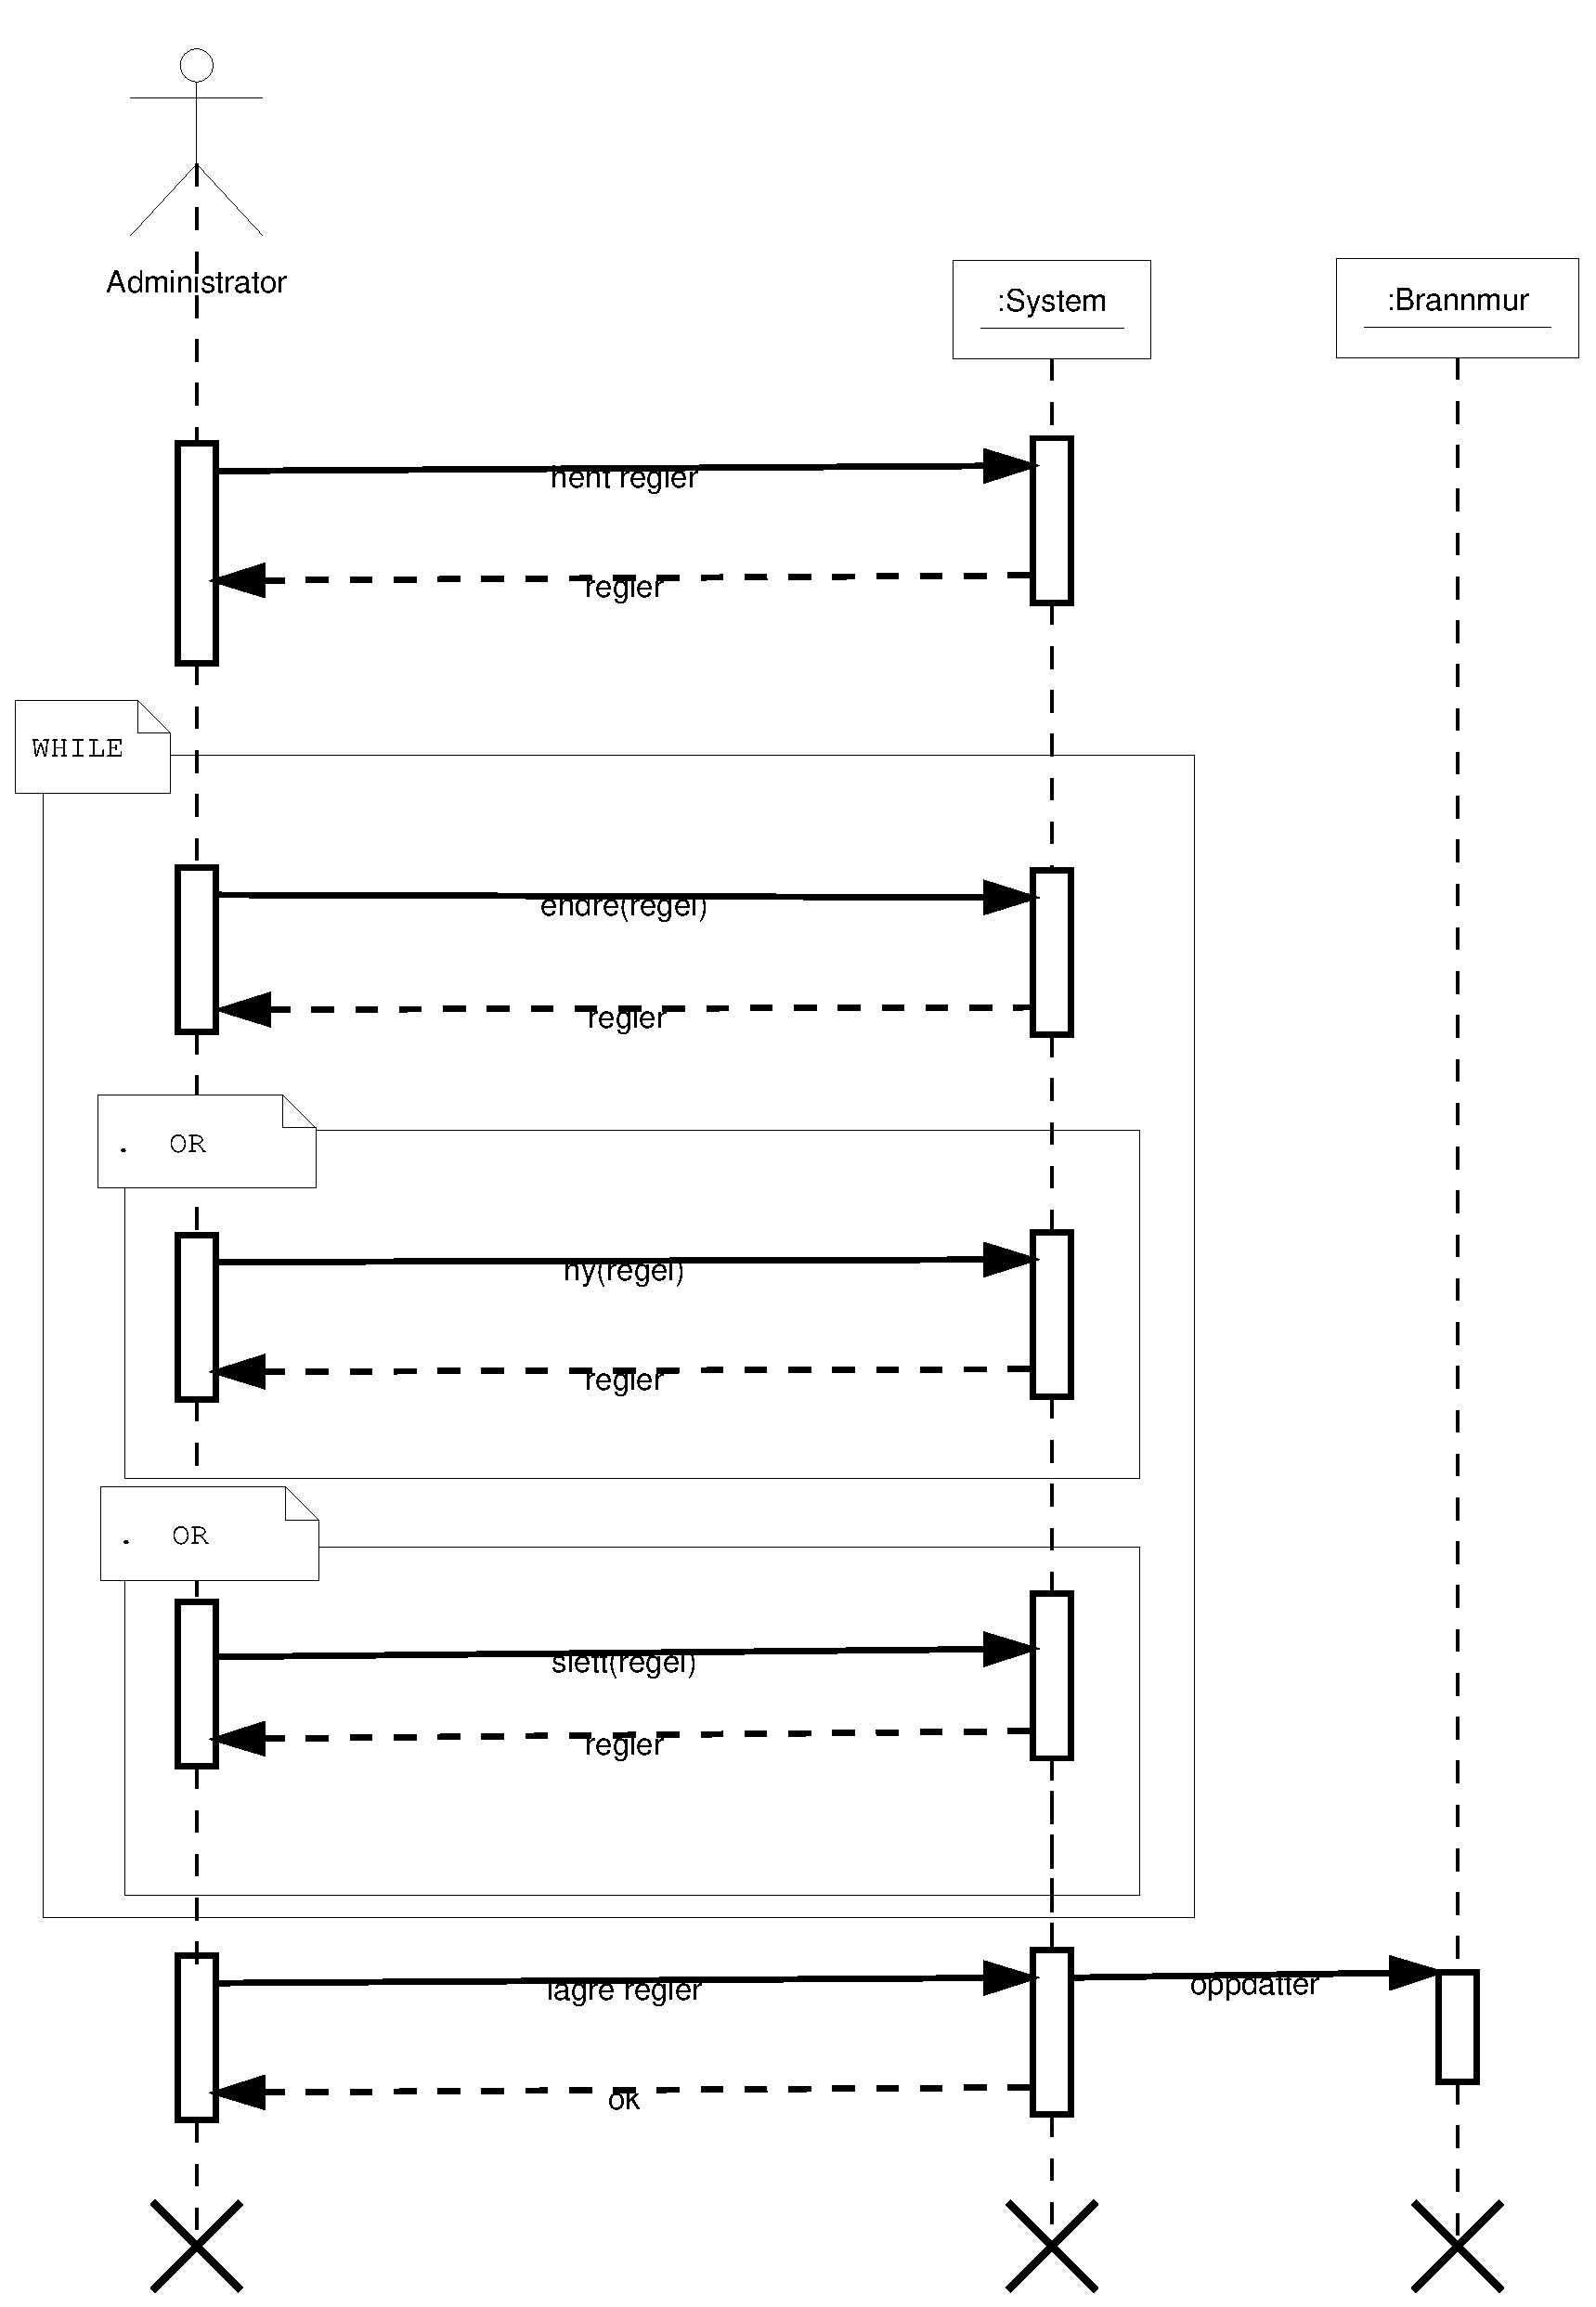
\includegraphics[scale=0.5]{gfx/SSD_UC3_administrer_brannmur.eps}

\newpage
\section{Problemdomenemodell}
\paragraph{}
Reglar kan enten være knytta til ein brukar, eller gjelde heile systemet. Ein brannmurregel har altså ein null til mange relasjon med brukarane.

\includegraphics[scale=0.5]{gfx/dm1.eps}
\end{document}
